\chapter{The Impact of AGN on Ly\texorpdfstring{$\alpha$}{a} Emission from Massive Halos}
\label{sec:agn}

We now turn our attention to the influence of AGN on our modeled Ly$\alpha$ emission.
Note that from the perspective if the hydrodynamic simulations, black holes are only implemented as sink particles without any feedback (\S~\ref{sec:methods}).
That is, though the black hole particles in this simulation will accrete mass, there is no prescription for the flow of thermal and kinetic energy into the surrounding gas from the accretion, which is what makes black holes astrophysically interesting in this context.
This should be contrasted with our use of an ionizing radiative transfer code to recompute the ionization state in postprocessing due to stars and the UV background.
In both cases this is not self-consistent, but in the previous cases there is already some approximation in the simulations for the energy contribution from these ionizing sources, wheras when we approximate an AGN, we are very self-inconsistent.
But that need not stop us from performing a numerical experiment in postprocessing; it only means that one needs to be cautious in interpreting the results of such an experiment.

Here, we treat AGN as an ionizing source when we compute the ionization state of the gas with {\sc lycrt}.
In this model, the AGN SED is modeled by employing the \citet*{Hopkins2007} templates for unreddened quasars, with the luminosity being tied to the accretion rate via $L = \eta \dot{M_{\rm BH}} c^2$, where $\eta$ is an efficiency parameter with a fiducial value of $\eta = 0.1$.
The impact of the chosen SED model is not particularly important in this work because we do not use it for the ionizing radiative transfer.
The SED informs the rate of ionizing photon emission that is given to {\sc lycrt}, but the emission that is actually used to compute the ionization state follows the aforementioned power law.
For most of this section, we will transform all of the black hole particles in the snapshots into sources for the ionization state calculation.
Sometimes this means there is a very impactful AGN in a satellite galaxy, not the central massive galaxy that the cosmological simulation is oriented around.
In what follows, we investigate the impact of AGN on the total Ly$\alpha$ luminosity, as well as the overall spatial extent of the blob and the blob morphology.

\section{Large-Scale Morphological Changes}
We include Figure \ref{fig:agn_rogues1}, \ref{fig:agn_rogues2}, \ref{fig:agn_rogues_4}, and \ref{fig:agn_rogues8} to orient the reader as to the visual effects of AGN on our model.
These figures contain half as many snapshots since we provide an exact side-by-side comparison of the halo with and without the AGN.
There is a remarkable consistency in terms of what changes; with the AGN present in the ionization state calculation the blobs appear smaller.
We also see some detail in them which was previously obscured; particularly at higher redshift there are bright regions which seem to have no counterpart in the images without AGN.
The trend in size is not exactly that these objects become smaller with AGN; looking closely one can see that there is more area occupied by the brighest regions.
That is, the overall change is to alter the distribution of surface brightness across the blob; the escape of Ly$\alpha$ has become more concentrated.

\begin{figure*}
    \centering
    \includegraphics[width=\textwidth,keepaspectratio]{figures/rogues_A1.png}
    \caption{
        Ly$\alpha$ surface brightness images of of halo A1 with and without AGN from $z=4.5$ (top-left) to $z=2.0$ (bottom-right).
        All images are 75$\times$75 physical kpc across, and are scaled from $2\times 10^{-19}-10^{-16}\ \rm{erg}\ \rm{s}^{-1}\ \rm{cm}^{-2}\ \rm{arcsec}^{-2}$.
    }
  \label{fig:agn_rogues1}
\end{figure*}

\begin{figure*}
    \centering
    \includegraphics[width=\textwidth,keepaspectratio]{figures/rogues_A2.png}
    \caption{
        Ly$\alpha$ surface brightness images of of halo A2 with and without AGN from $z=4.5$ (top-left) to $z=2.0$ (bottom-right).
        All images are 75$\times$75 physical kpc across, and are scaled from $2\times 10^{-19}-10^{-16}\ \rm{erg}\ \rm{s}^{-1}\ \rm{cm}^{-2}\ \rm{arcsec}^{-2}$.
    }
  \label{fig:agn_rogues2}
\end{figure*}

\begin{figure*}
    \centering
    \includegraphics[width=\textwidth,keepaspectratio]{figures/rogues_A8.png}
    \caption{
        Ly$\alpha$ surface brightness images of of halo A8 with and without AGN from $z=4.5$ (top-left) to $z=2.0$ (bottom-right).
        All images are 75$\times$75 physical kpc across, and are scaled from $2\times10^{-19}-10^{-16}\ \rm{erg}\ \rm{s}^{-1}\ \rm{cm}^{-2}\ \rm{arcsec}^{-2}$.
    }
  \label{fig:agn_rogues8}
\end{figure*}

\begin{figure*}
    \centering
    \includegraphics[width=\textwidth,keepaspectratio]{figures/rogues_A4.png}
    \caption{
        Ly$\alpha$ surface brightness images of of halo A4 with and without AGN from $z=4.5$ (top-left) to $z=2.0$ (bottom-right).
        All images are 75$\times$75 physical kpc across, and are scaled from $2\times10^{-19}-10^{-16}\ \rm{erg}\ \rm{s}^{-1}\ \rm{cm}^{-2}\ \rm{arcsec}^{-2}$.
    }
  \label{fig:agn_rogues4}
\end{figure*}


\section{Impact of AGN on Luminosity and Escape Fraction}
In Figure~\ref{fig:agn_recombination_collision} we plot the escaping and intrinsic luminosity due to recombinations and collisions with our approximation for the effects of AGN.
In all cases, we see an increase in emission due to recombinations, and a decrease in emission due to collisional excitation.
Unlike many other observations in this section; this is unsurprising: A gas that experiences a more intense UV field is more ionized and thus favors emission by recombinations (\S~\ref{sec:physicalconcepts}).

As in Figure~\ref{fig:recombination_collision}, the distance between the pale and darker lines provides a visualization of the escape fraction along a median line of sight.
In this case, there is a clear redshift evolution of the escape fraction due to recombinations.
Towards $z=5$, the the escape fraction is very close to $1$, and as the halo evolves it decreases.
This could be explained as a direct consequence of self-shielding and the growth of halo mass over time.
At high redshift, the gas which is ionized by the AGN and thus accounts for the increase in recombination luminosity is directly exposed to observer outside the halo.
Over time, neutral gas accumulates around the AGN and the ionizing luminosity is increasingly insufficient to ionize large pathways through scattering gas, and thus the Ly$\alpha$ is scattered through more dust and partly absorbed.

This story contrasts strongly with the behavior of the collisional emission in these halos.
This source is suppressed by the presence of an AGN, though the effect is not as significant as the enhancement of recombination emission.
There is also an effect on the escape fraction, but it is more complicated to interpret.
The escape fraction of Ly$\alpha$ is linked to the opacity of the gas because both depend in $n_{\rm{HI}}$.
Unlike the emission due to recombinations which is preferentially emitted in ionized regions, emission due to collisional excitations is preferentially emitted in neutral regions, where the local optical depth is high and thus such photons are more likely to be scatterd and absorbed before they escape the domain.

There is one more question raised by Figure~\ref{fig:agn_recombination_collision} we would like to answer: Why doesn't the recombination luminosity grow over redshift?
We know that the mass of all AGN in the simulation grow, and since their luminosities in our simulation are tied only to the mass, their ionizing output grows proportionally, but we can see from this figure that the Ly$\alpha$ luminosity that this drives does not grow.
A precise explanation of this is worth much more study, but for now we can offer a few explanations.
It is possible that as the mass of the black hole grows, the system becomes more radially asymmetric (possibly because it is settling into a disk) which would reduce the covering fraction of the black hole, and more of the ionizing flux would not go into ionizing the surrounding gas.
It is also possible that in this scenario the luminosity of the halo is not particularly sensitive to the ionizing luminosity of the AGN, which would be possible if the AGN has ionized essentially all of the gas except for a few small pockets of very self-shielded gas.
This explanation is supported by the dramatic drop in luminosity due to recombinations, and some of the results in \S~\ref{sec:ionization_extremes}.

\begin{figure}
    \centering
    \includegraphics[width=\textwidth,height=\textheight,keepaspectratio]{figures/agn_recombination_collision.pdf}
    \caption{
        All our snapshots broken down by source of emission over redshift; as opposed to Figure~\ref{fig:recombination_collision} this plot includes the effect of AGN.
    }
    \label{fig:agn_recombination_collision}
\end{figure}

Previously in section \S~\ref{sec:los} that Ly$\alpha$ escape can have a strong line-of-sight dependence, and explained why that can be and what sorts of geometries can arise.
With the presence of AGN in our model all these effects become more dramatic, as we show in Figure~\ref{fig:agn_los}.
The most striking feature in this plot is the much greater dependence on line of sight with AGN (though we do also see a net increase in escape fraction this has been discussed previously).
This huge variation when AGN are present is caused by the distinct non-uniformity of CGM opacity; it's as if the AGN punches large ionization holes in the enclosing CGM through which Ly$\alpha$ readily escapes.
There are two features in these plots that deserve specifc explanation: At some redshifts the escape fraction range of the AGN model extends below the no-AGN model, and at some redshifts the median escape fraction with AGN passes below that of the no-AGN model.
These are surprising for the same reason: the effect of the AGN is to ionize more gas, which reduces the opacity of the halo... So how could this sometimes cause less Ly$\alpha$ to escape?

For the first case, where some lines of sight see a lower escape fraction, we present an example scenario in Figure~\ref{fig:scattering_diagram}, where the star represents a source of Ly$\alpha$, the color of the box represents the ionization state of the gas, and the light gray circle represents a dense region of neutral gas.
In the no-agn case, Ly$\alpha$ emitted in the direction of the observer towards this dense region of gas, but scatters off it.
However this Ly$\alpha$ does not (or does not all) escape traveling away from the observer.
Since it is passing through gas which is only partly ionized, there is a probability that it will be scattered back towards the observer and enter the dense region, and eventually escape in the direction of the observer.
In the right panel, when an AGN is present, the gas around this dense region is fully ionized and thus Ly$\alpha$ which scatters off the dense region will never be seen by the observer.
But more importantly since the Ly$\alpha$ which scatters off this has no neutral hydrogen between it and the edge of the simulation domain the net escape fraction is elevated, even though an observer looking towards the source from the bottom of the page sees much less Ly$\alpha$ escape towards their line of sight.

In the second scenario, where the median escape fraction with AGN on dips below the escape fraction without AGN the explanation, the previous explanation does not apply.
In that scenario we needed to invoke a small and dense self-shielded parcel of gas along the particular line(s) of sight with low escape fraction, but in this scenario we see a decreased escape fraction along at least half of all lines of sight.
The explanation we offer for this scenario is unfortunately more subtle.
Recall that the escape fraction is the ratio of escaping Ly$\alpha$ to emitted Ly$\alpha$, so while we mostly focus on the escape process it is sufficient to alter the amount of emitted Ly$\alpha$ if doing so does not alter as much the amount of Ly$\alpha$ that escapes.
Alternatively, we can view an escape fraction as a luminosity-weighted integral of the escape fraction of all positions in the simulation.
Thus because of the weighting if the luminosity is disproportionately increased in cells which have low escape fractions (that is, low escape fractions out of the entire simulation, not to neighboring cells), we can decrease the escape fraction of the simulation as a whole, even though the luminosity along that line of sight may increase.


\begin{figure}
    \centering
    \includegraphics[width=\textwidth]{figures/scattering_diagram.png}
    \caption{
        A schematic of a scenario in which one line of sight (observer at the bottom of the page) may see a lower escape fraction with an AGN and thus a greater ionization fraction.
    }
    \label{fig:scattering_diagram}
\end{figure}

\begin{figure}
    \centering
    \includegraphics[width=\textwidth,height=\textheight,keepaspectratio]{figures/agn_los.pdf}
    \caption{
        A single snapshot, seen from 12 equally spaced lines of sight.
    }
    \label{fig:agn_los}
\end{figure}



% TODO: Continue here


\begin{figure}
    \centering
    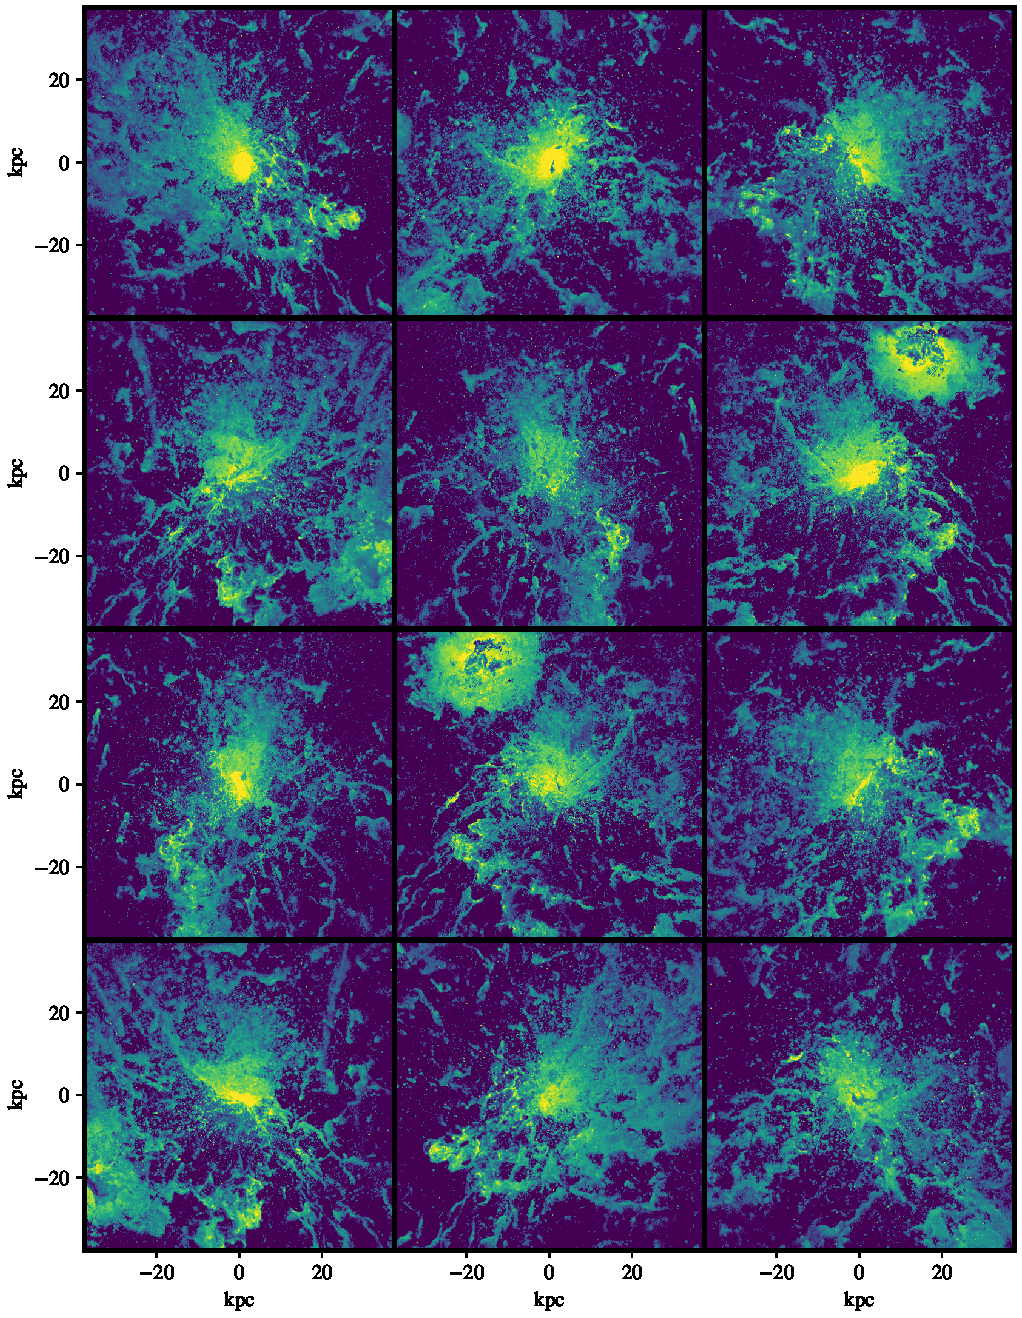
\includegraphics[width=\textwidth,height=\textheight,keepaspectratio]{figures/many_los.pdf}
    \caption{
        A single snapshot, seen from 12 equally spaced lines of sight.
    }
    \label{fig:many_los}
\end{figure}


% TODO: Update to Gini coefficient discussion
\section{The impact of AGN on the spatial extent and concentration of Ly\texorpdfstring{$\alpha$}{a} in blobs}

As in the overall Ly$\alpha$ luminosity, the AGN can also impact the spatial extent of Ly$\alpha$ emission in massive halos.
This takes two forms: (1) the total area enclosed within a surface brightness contour and (2) the concentration of Ly$\alpha$ light in the system.
We explore these in turn.

Previously, in Figure~\ref{fig:area_plot}, we examined the size of our model LABs as a function of observation sensitivity (solid lines) in a fiducial model that did not have AGN on.
We now turn to the dashed lines in the same figure where we have included AGN.

We see an enhancement of blob size at high surface brightness cutoffs, which indicates that there are regions that have been substantially enhanced in brightness, but at the same time we see a decrease in blob size at much lower cutoffs.
We interpret this effect as a complex interaction of the gas ionization state with escape pathways.
As gas becomes more ionized it provides a pathway along which Ly$\alpha$ is likely to escape; it is these pathways that produce the small region(s) of very intense surface brightness.
However, the presence of a low-opacity pathway out of the blob decreases the probability that a photon will be scattered out into the extended blob structure before it escapes.

The presence of these small pathways out of blob may be useful to detect the presence of AGN in a blob.
We quantify the concentration of light via a metric analogous to $M_{\rm 20}$ \citep{Lotz2004}, where we compute the fraction of pixels in our surface brightness images containing half the total flux, shown for all our snapshots in Figure~\ref{fig:skewness}.
The primary signature of the AGN's effect is to cause the luminosity to be concentrated in a much smaller area.
While this may seem contradictory to the increase in total luminosity and area enclosed, note that this is a {\it relative} concentration.
That is, while the diffuse emission is still significant, the central emission in the ionized bubble surrounding the AGN dominates when compared to this diffuse halo emission such that the overall concentration decreases dramatically for the AGN-on model.
This metric becomes more effective for identifying AGN with higher-resolution observations (Figure~\ref{fig:MUSE}); the bright patches of our surface brightness images are significantly smaller than the spatial resolution of current telescopes.

\begin{figure}
    \centering
    \includegraphics[width=\textwidth,height=\textheight,keepaspectratio]{figures/141.pdf}
    \caption{
        Example surface brightness image of a LAB where the luminosity is concentrated, which indicates the presence of an AGN, but the luminosity is not in a connected region.
    }
    \label{fig:agn_on_example}
\end{figure}

\begin{figure}
    \centering
    \includegraphics[width=\textwidth,height=\textheight,keepaspectratio]{figures/skew_distribution.pdf}
    \caption{
        We propose a metric for determining the presence of an AGN in an observed LAB: The fraction of all flux that is concentrated within a small fraction of the total area of the blob.
    In this figure since we are making a suggestion for an observable metric we have computed this metric on simulated surface brightness images after convolving to the resolution of MUSE.
    For the purpose of this demonstration we plot the fraction of pixels containing 50\% total flux but one could choose another threshold and find similar results.
    }
    \label{fig:skewness}
\end{figure}

\section{Impact of AGN model}
